\documentclass[11pt,a4paper]{article}
\usepackage[utf8]{inputenc}
\usepackage[german]{babel}
\usepackage[T1]{fontenc}
\usepackage{amsmath}
\usepackage{amsfonts}
\usepackage{amssymb}
\usepackage{graphicx}
\usepackage[margin=1.25cm]{geometry} % Puts the same margin on all borders of the document

% Packages

\usepackage{hyperref} % Generate hyperlinks to referenced items
\usepackage{adjustbox} % Used to change parameters in \includegraphics[scale=•]{•}
\usepackage{enumitem} % Provides several options for lists
\usepackage{verbatim} % Package to use \begin{comment}
\usepackage{pdfpages} % Used to import PDF pages
\usepackage{multirow} % Allows us to have a single cell in a table span multiple rows
\usepackage{makecell} % Allows us to format multiple lines in a single cell
\usepackage{minted} % Used to syntax highlight code
\usepackage{xcolor}  % Gives access to coloring text
\usepackage{longtable} % Allows us to create a table over multiple pages
\usepackage{float} % Improved placement of floating items
\usepackage{pdfpages} % Used to import pdf pages
\usepackage{booktabs} % Used for horizontal lines instead of \hline



% Settings

\graphicspath{{./files/}} % Sets path for files to the files folder in the same directory

\hypersetup{
    colorlinks=false, %set true if you want colored links
    linktoc=all,     %set to all if you want both sections and subsections linked
    linkcolor=blue,  %choose some color if you want links to stand out
}

\tcbuselibrary{minted,skins}

\definecolor{vlcodebg}{rgb}{0.85,0.85,0.85}

% Kudos an Rubos
% code environment with boxes
\newtcblisting{ccode}[2][]{
    listing engine=minted,
    colback=vlcodebg!30, 
    colframe=black!70,
    listing only,
    %minted style=colorful,
    minted language=c,
    minted options={ 
      linenos=true,
      numbersep=3mm,
      texcl=true,
      #1 
      },
      left=5mm,
      enhanced,
      overlay={
                \begin{tcbclipinterior}
                  \fill[black!25] (frame.south west) rectangle ([xshift=5mm]frame.north west); % Zeilennummernbereich färben
                \end{tcbclipinterior}
              },
      #2
}

\begin{titlepage}
    \title{AUD Klausurblatt SoSe 2020 | Janson/Fischlin} % document_name-type_of_document
    \author{J. Milkovits}
    \date{Last Edited: \today}
  \end{titlepage}
  
  \begin{document}
  
  \pagenumbering{gobble}
  \maketitle
  \vspace{2cm}
  \centerline{{\Large \textbf{Empfehlung: Titelblatt dient nur zur Übersicht, für Klausur lieber Post-Its!}}}
  \vspace{2cm}
  \pagenumbering{roman} % i, ii, iii on beginning pages, that don't have content
  \tableofcontents

  \clearpage
  \pagenumbering{arabic} % 1,2,3 on content pages


\begin{center}
    {\huge \textbf{AUD Klausurblatt SoSe 2020 | Janson/Fischlin}}
\end{center}

\section{Definitionen/Wissen}
    \subsection{Master-Theorem}
        \begin{itemize}
            \item \textit{Anwendbar?}
                \begin{itemize}
                    \item $a \geq 1$ und konstant?
                    \item $b > 1$ und konstant?
                    \item $f(n)$ positiv?
                \end{itemize}
            \item \textit{Vorgehen}
                \begin{itemize}
                    \item Berechnung von $log_b(a)$
                    \item Vergleich mit $f(n)$
                        \begin{itemize}
                            \item {\makebox[8cm][l]{$f(n)$ \textbf{polynomial kleiner} als $n^{log_b(a)}$}}  $\Rightarrow$ $T(n) = \Theta(n^{log_b(a)})$
                            \item[] $(f(n) = O(n^{log_b(a-\epsilon)})$, $\epsilon > 0$)
                            \item {\makebox[8cm][l]{$f(n)$ und $n^{log_b(a)}$ \textbf{gleiche Größe}}}  $\Rightarrow$ $T(n) = \Theta(n^{log_b(a)} lg(n))$
                            \item[] $(f(n) = \Theta(n^{log_b(a)})$
                            \item {\makebox[8cm][l]{$f(n)$ \textbf{polynomial größer} als $n^{log_b(a)}$ und}} 
                            \item[] {\makebox[8cm][l]{$af(\frac{n}{b}) \leq c~f(n)$, ($\epsilon < 1)$}}  $\Rightarrow$ $T(n) = \Theta(f(n))$
                            \item[] ($f(n) = \Omega (n^{log_b(a + \epsilon)})$, $\epsilon > 0$) 
                        \end{itemize}
                \end{itemize}
        \end{itemize}

    \subsection{Asymptotik}
        \begin{itemize}
            \item $\frac{f(n)}{g(n)} = 0$ $\Rightarrow$ $f(n) = o(g(n))$
            \item $\frac{f(n)}{g(n)}: konvergent$ $\Rightarrow$ $f(n) = O(g(n))$
            \item $o(n) \in O(n)$ $\Rightarrow$ schließt alle anderen aus
            \item $f(n) = g(n)$ $\Rightarrow$ $f(n) = \Theta(g(n))$
        \end{itemize}

    \subsection{Sortier-Algorithmen in einem Satz}
        \begin{itemize}
            \item \textit{InsertionSort}: Sortierthalten der linken Teilfolge, neuen Wert an richtige Position einfügen
            \item \textit{BubbleSort}: Vergleiche Paare von benachbarten Schlüsselwerten
            \item \textit{SelectionSort}: Wähle kleinstes Element und tausche es nach vorne
            \item \textit{MergeSort}: Teilen, sortiertes Zurückschreiben in Array
            \item \textit{QuickSort}: Vergleich der Werte mithilfe PivotElement, rekursiver Aufruf auf Teilarray
        \end{itemize}

    \subsection{Bäume in einem Satz}
        \begin{itemize}
            \item \textit{BinarySearchTree}: Suchbaum mit Ordnung auf Werten (kleinere Werte links, größere rechts)
            \item \textit{RedBlackTree}: BST mit Zusatzeigenschaften (Rot/Schwarz, Root: Schwarz, Nicht-Rot-Rot, Schwarzhöhe)
            \item \textit{AVL}: BST, Teilbäume müssen jedoch balanciert sein (Unbalance maximal -1, 1)
            \item \textit{Splay}: BST, selbst organisierende Liste (angefragte/neue Werte werden nach oben gespült)
            \item \textit{Max-Heaps}: Kein BST, vollständig gefüllt (links -> rechts), Maximum in Wurzel, Parent > Child
            \item \textit{B-Trees}: Kein BST, angegebener Grad, der die Fülle jedes Knotens bestimmt, Ordnung zwischen Knoten
        \end{itemize}

    \subsection{Advanced Designs}
        \subsubsection{Dynamische Programmierung}
            \begin{itemize}
                \item Anwendung, wenn Teilprobleme sich überlappen
                \item bereits gelöste Teilprobleme werden gespeichert und bei Bedarf nachgeschlagen
                \item Laufzeit-Speicher-Tradeoff
                \item Memoisation: Wert der Berechung speichern, um obiges zu verhindern
                \item Bottom-Up: Löst immer zuerst die kleinen Teilprobleme und arbeitet sich von unten nach oben
                \item Top-Down: Arbeitet sich von großen zu kleinen Problemen
            \end{itemize}

        \subsubsection{Greedy-Algorithmus}
            \begin{itemize}
                \item Trifft stets die Entscheidung, die im Moment am besten erscheint
                \item lokale Optimierung in der Hoffnung auf globale Optimierung
                \item Aktivitätenauswahl mit Greedy:
                    \begin{itemize}
                        \item Wahl der Aktivität mit geringster Endzeit (möglichst viele freie Resourcen)
                        \item Ab dort rekursiv weiter
                    \end{itemize}
            \end{itemize}

        \subsubsection{Backtracking}
            \begin{itemize}
                \item Lösen via Trial and Error / Schrittweises Herantasten an die Gesamtlösung
                \item Falls Teillösung inkorrekt $\rightarrow$ Schritt zurück und andere Möglichkeit
                \item Voraussetzung: Komponentenlösung / Mehrere Wahlmöglichkeiten / Teillösung verifizierbar
            \end{itemize}

        \subsubsection{Optimierungsproblem - Metaheuristiken}
            \begin{itemize}
                \item Finden einer Lösung und Überprüfen dieser
                \item Danach versuche eine bessere Lösung (Finde globales Maxima) in der Nachbarschaft zu finden
                \item \textit{Zufällige Suche}
                    \begin{itemize}
                        \item Falls zufällige Lösung besseren Wert als aktuelle Lösung hat, übernimm Lösung und wiederhole dies
                        \item[+] \textbf{kann} im globalen Optimum terminieren
                        \item[-] potentiell lange Laufzeit 
                    \end{itemize}
                \item \textit{Bergsteigeralgorithmus}
                    \begin{itemize}
                        \item Iterative Verbesserungstechnik
                        \item Auswahl einer neuen zufälligen Lösung aus Nachbarschaft
                        \item Falls diese besser ist wird sie übernommen $\rightarrow$ wiederholen
                        \item[+] einfach anzuwenden
                        \item[-] terminiert in der Regel bei lokalem Optimum 
                    \end{itemize}

                \item \textit{Iterative lokale Suche}
                    \begin{itemize}
                        \item Sucht Lösungen nur in einem bestimmten Bereich mit Bergsteigeralgorithmus
                        \item Springt aber dann weiter weg (aus Nachbarschaft raus) um anderes Optimum zu finden
                    \end{itemize}
\pagebreak
                \item \textit{Simulated Annealing}
                    \begin{itemize}
                        \item Wie Bergsteigeralgorithmus, wählt aber mit gewisser Wahrscheinlichkeit auch schlechtere Lösungen
                        \item Auch mit Tabu-List (speichert bereits verwendete Lösungen) umsetzbar
                    \end{itemize}

                \item \textit{Evolutionary}
                    \begin{itemize}
                        \item Hier wird eine Stichprobe von möglichen Lösungen betrachtet (populationsbasiert)
                        \item Generiert zufällige Populationen, beurteilt die Qualität jedes Individuums
                        \item Löscht dann die schlechtesten Individuuen und ersetzt diese durch neue
                    \end{itemize}
            \end{itemize}

        \subsubsection{Amortisierte Analyse}
            \begin{itemize}
                \item Genauere Abschätzung des Worst-Case von Algorithmen
                \item Wie? Nicht alle Operationen sind gleichteuer $\rightarrow$ genauere Abschätzung
                \item[] (z.B. abhängig vom aktuellen Zustand der Datenstruktur)
                \item[] $\Rightarrow$ Ermittlung der mittleren Perfomanz jeder Operation im Worst-Case
                \item \textit{Aggregat-Methode}: Aufsummation der tatsächlich anfallenden Kosten aller Operationen
                \item \textit{Account-Methode}: Besteuerung und Zuweisung höherer Kosten an Operationen, Guthabenmodell
                \item \textit{Potential-Methode}: Betrachtung des Einflusses auf die Datenstruktur durch Operationen 
            \end{itemize}

    \subsection{NP}
        \begin{itemize}
            \item Sind alle Probleme in polynomieller Zeit lösbar? ($O(n^k)$)
            \item[] $\Rightarrow$ Nein, manche nur in superpolynomieller Zeit lösbar ($k^n$)
            \item \textit{P}: 
            \begin{itemize}
                \item Klasse aller Polynomialzeitprobleme (in polynomieller Zeit lösbar)
                \item Betrachtung von Optimierungsprobleme $\rightarrow$ bestimmter Wert
                \item Optimierungsprobleme oft in Entscheidungsprobleme umwandelbar (Schranke für Ergebnis)
                \item $P \subseteq NP$
            \end{itemize} 
            \item \textit{NP}: 
                \begin{itemize}
                    \item Alle Probleme, der Lösung in Polynomialzeit \textbf{verifizierbar} ist
                    \item Betrachtung von Entscheiduzngsprobleme $\rightarrow$ Ja/Nein
                    \item Für viele wichtige Probleme unbekannt, ob sie in $P$ (effizient) lösbar sind
                    \item \textit{NP-Schwer}: Vergleich mit anderen $NP$-Problemen (mindestens genauso schwierig)
                    \item \textit{NP-Vollständig}: Sowohl $NP$-schwer als auch in $NP$
                \end{itemize}
        \end{itemize}
\pagebreak
    \subsection{String-Matching}
        \subsubsection{Allgemein}
            \begin{itemize}
                \item {\makebox[4cm][l]{durchsuchender Text:}}  Array \texttt{T} der Länge \texttt{lenTxt}
                \item {\makebox[4cm][l]{Textmuster:}}  Array \texttt{P} der Länge \texttt{lenPat $\leq$ lenTxt}
                \item {\makebox[4cm][l]{Gesucht:}}  alle gültigen Verschiebungen mit denen \texttt{P} in \texttt{T} auftaucht
                \item {\makebox[4cm][l]{Rückgabe:}} alle \texttt{sft $\in \mathbb{N}$}, sodass \texttt{T[sft,$\dots$,sft+lenPat-1] = P} gilt
            \end{itemize}

        \subsubsection{NaiveStringMatching}
            \begin{minipage}{0.4\textwidth}
                \textit{Pseudocode:}
                \begin{ccode}[autogobble,escapeinside=||]{title={NaiveStringMatching(T,P)}}
                lenTxt = length(T)
                lenPat = length(P)
                L = empty
                FOR sft = 0 TO lenTxt - lenPat DO
                    isValid = TRUE
                    FOR j = 0 TO lenPat - 1 DO
                        IF P[j] |$\neq$| T[sft+j] THEN
                            isValid = FALSE
                    IF isValid THEN
                        L = append(L, sft)
                RETURN L
                \end{ccode}
            \end{minipage}
            \begin{minipage}{0.5\textwidth}
                \textit{Beispiel:} \texttt{T=[h,e,h,e,h,h,h,e,y,h]}, \texttt{P=[h,e,h]} \\
                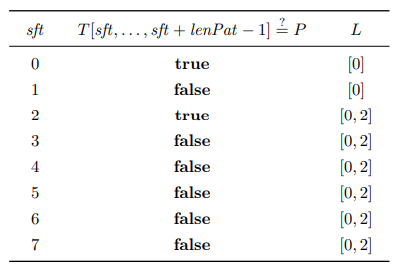
\includegraphics[height=6.5cm]{naiveStringMatchingBsp.png}
            \end{minipage}

        \subsubsection{FiniteAutomationMatching}
            \textit{Pseudocode:}
            \begin{ccode}[autogobble,escapeinside=||]{title={FiniteAutomationMatching(T, $\delta$, lenPat)}}
            lenTxt = length(T)
            L = empty
            st = 0
            FOR sft = 0 TO lenTxt - 1 DO
                st = |$\delta$|(st, T[sft])
                IF st = lenPat THEN
                    L = append(L, sft - lenPat + 1)
            RETURN L
            \end{ccode}

            \noindent
            \textit{Beispiel:} \texttt{$\Sigma$ = \{a,b\}}, \texttt{P = [a,b,a,a]}, \texttt{T = [a,a,b,a,b,a,a,b,a,a]} \\
            \centerline{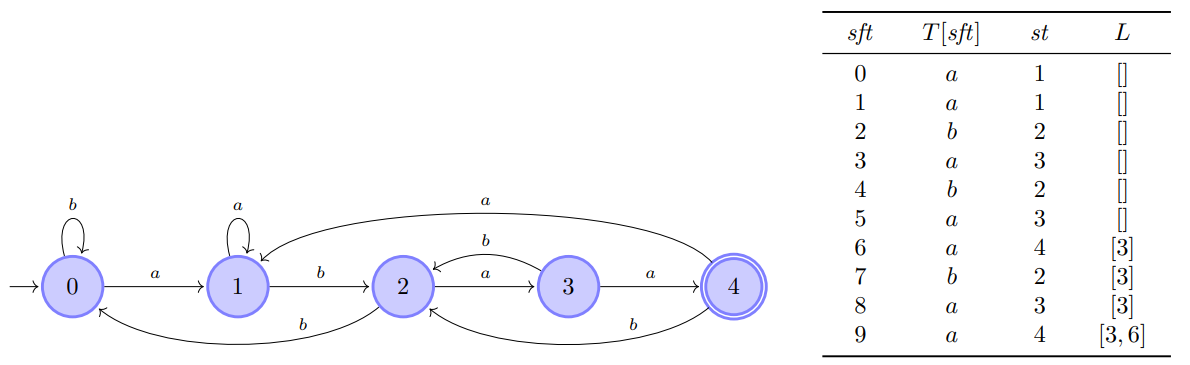
\includegraphics[width=15cm]{finiteAutomationMatching.png}}
\pagebreak
        \subsubsection{Rabin-Karp-Algorithmus}

            \textit{Pseudocode:}
            \begin{ccode}[autogobble,escapeinside=||]{title={RobinKarpMatch(T,P,q)}}
            n = T.length
            m = P.length
            h = |$10^{m-1}$| (mod q)
            p = 0, |$t_0$| = 0, L = empty
            FOR i = 0 TO m-1 DO
                p = (10p + P[i]) (mod q)
                |$t_0$| = (10|$t_0$| + T[i]) (mod q)
            FOR s = 0 TO n - m DO
                IF p == |$t_s$| THEN
                    b = TRUE
                    FOR j = 0 TO m - 1 DO
                        IF P[j] |$\neq$| T[s+j] THEN
                            b = FALSE
                            BREAK
                    IF b THEN
                        L.add(s)
                IF s < n - m THEN
                |$t_{s+1}$| = (10(|$t_s$| - T[s]h) + T[s+m]) (mod q)
            RETURN L
            \end{ccode}

            \noindent
            \textit{Beispiel}: \texttt{P = [7,3,4]}, \texttt{T = [6,9,1,7,3,4,5,0,9,4,6,2,4,8,7,3,4]}, \texttt{q = 13}, Ergebnis \texttt{L = [3,14]} \\
            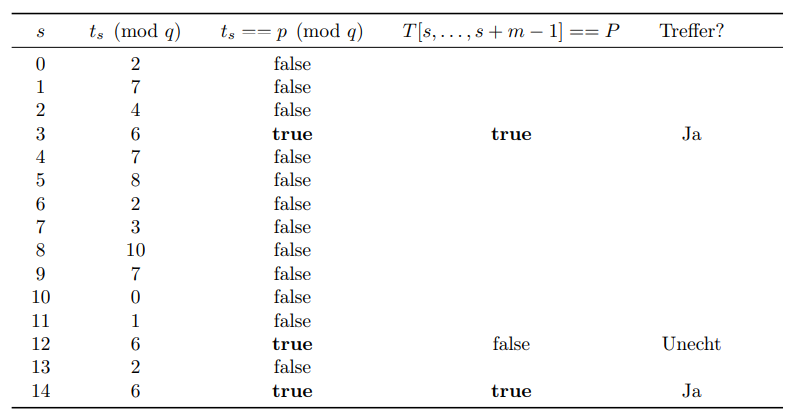
\includegraphics[width=12cm]{rabinKarpBsp.png}




    \subsection{Queue mithilfe von zwei Stacks}

        $enqueue$ pusht auf den ersten Stack. \\
        $dequeue$ wird als $pop(S_2)$ definiert. \\
        Falls der zweite Stack leer ist werden alle Elemente aus $S_1$ geholt und in $S_2$ überführt. \\
        Dann wird das erste Element von $S_2$ ausgegeben. \\
        \centerline{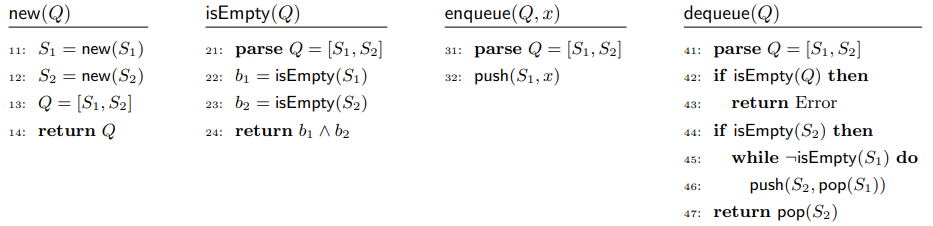
\includegraphics[width=12cm]{stackQueue.png}}
\pagebreak
    \subsection{Stack mithilfe von zwei Queues}

        Eine der beiden Queues bleibt immer leer (anfangs $Q_2$) \\
        $push$ fügt Wert immer der leeren Queue hinzu. \\
        $pop$ holt alle Elemente bis auf das letzte aus der Queue zurück und fügt sie in die leere ein. \\
        Das letzte Element wird dann ausgegeben. \\
        \centerline{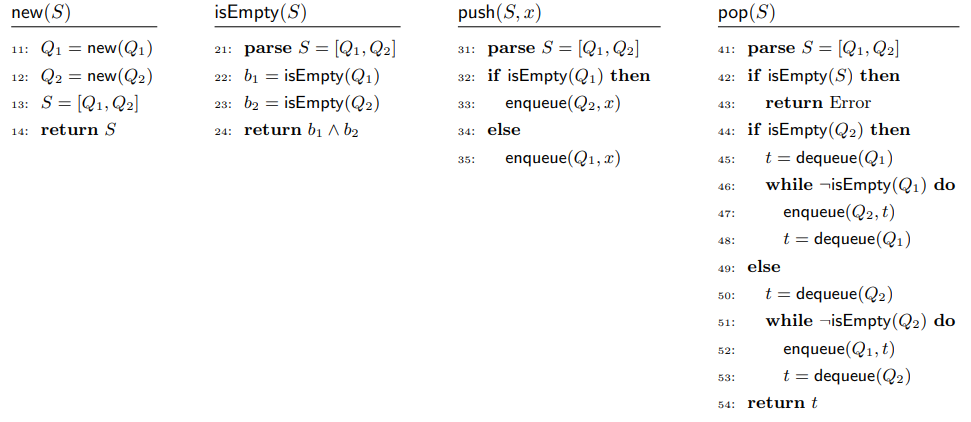
\includegraphics[width=12cm]{queueStack.png}}

    \subsection{Graphen - Adjazenzmatrix/-liste}
        \begin{minipage}{0.45\textwidth}
            \textit{Umformung Liste $\rightarrow$ Matrix}
            \begin{ccode}[autogobble, escapeinside = ||]{title={listToMatrix(L)}}
                nNodes = length(L)
                M = newMatrix(nNodes, nNodes, 0)
                FOR i = 0 to nNodes - 1 DO
                    node = L[i]
                    WHILE node |$\neq$| nil DO
                        j = node.key
                        M[i,j] = 1
                        node = node.next
                RETURN M
            \end{ccode}
        \end{minipage}
        \begin{minipage}{0.45\textwidth}
            \textit{Umformung Matrix $\rightarrow$ Liste}
            \begin{ccode}[autogobble, escapeinside = ||]{title={matrixToList(M)}}
                nNodes = rows(M)
                L = newArray(nNodes)
                FOR i = 0 to nNodes - 1 DO
                    L[i] = newList()
                    FOR j = 0 TO nNodes - 1 DO
                        IF M[i,j] = 1 THEN
                            insert(L[i],j)
                RETURN L
            \end{ccode}
        \end{minipage}

    

    \subsection{Graphenalgorithmen}
        \subsubsection{Breadth-First-Search}
            \begin{itemize}
                \item Besuche zuerst alle unmittelbaren Nachbarn, dann deren Nachbarn, usw.
                \item Funktionsweise:
                    \begin{itemize}
                        \item setzt alle Knoten auf Weiß und Distanz auf $+\infty$
                        \item Startknoten grau, Distanz grau, Vorgänger nil
                        \item Fügt alle Nachbarn einer Queue hinzu die weiß sind und passt deren Distanz an (dist+1)
                        \item Setzt Knoten auf Schwarz, wenn alle Nachbarn hinzugefügt und holt sich neuen Knoten aus Queue
                    \end{itemize}
            \centerline{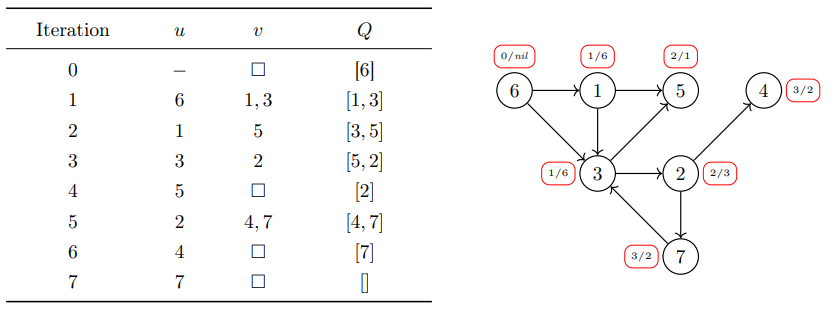
\includegraphics[width=10cm]{bfsBsp.png}}
            \end{itemize}
\pagebreak
        \subsubsection{Depth-First-Search}
            \begin{itemize}
                \item Besuche zuerst alle noch nicht besuchten Nachfolgeknoten
                \item \string"Laufe so weit wie möglich weg vom aktuellen Knoten\string"
                \item \textit{Funktionsweise DFS (Initialaufruf):}
                    \begin{itemize}
                        \item Setzt alle Knoten auf Weiß, Vorgänger auf nil, time auf 0
                        \item Ruft innerhalb einer for-Schleife auf jedem Knoten DFS-VISIT auf
                    \end{itemize}
                \item \textit{Funktionsweise DFS-Visit:}
                    \begin{itemize}
                        \item Wird min. einmal auf jedem Knoten aufgerufen
                        \item Erhöht zuallererst time um 1
                        \item setzt discovery time der Node auf time und Farbe auf grau
                        \item Ruft innerhalb For-Schleife für jeden weißen Nachbarn DFS-Visit auf
                        \item Falls die rekursive For-Schleife abgeschlossen ist -> Node Schwarz / time + 1
                        \item Abspeichern der finish-Zeit (u.finish = time)
                    \end{itemize}
                \item[]
                    \begin{minipage}{0.3\textwidth}
                        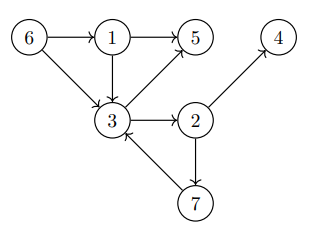
\includegraphics[height=3cm]{dfsBsp2.png}
                    \end{minipage}
                    \begin{minipage}{0.45\textwidth}
                        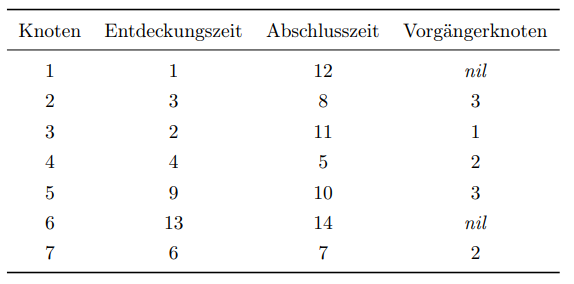
\includegraphics[height=3cm]{dfsBsp1.png}
                    \end{minipage}
                \item \textit{Anwendungen DFS: \texttt{Topo-Sort}}
                    \begin{itemize}
                        \item nur für directed acyclic graphs
                        \item Kanten zeigen immer nur nach rechts
                        \item (alternativ: führe DFS aus und schreibe Werte auf - starte bei höchster finish time)
                        \item[]
                            \begin{ccode}[autogobble]{title={TOPOLOGICAL-SORT(G)}}
                                newLinkedList(L)
                                run DFS(G) but, each time a node is finished, insert in front of L
                                RETURN L.head
                            \end{ccode}
                        \item[] \centerline{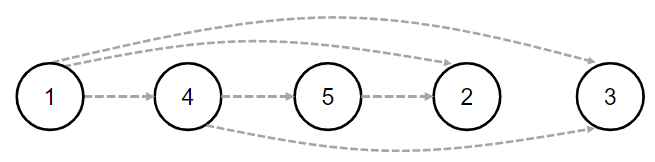
\includegraphics[width=9cm]{topo.png}}
                    \end{itemize}
                \item \textit{Starke Zusammenhangskomponenten}
                    \begin{itemize}
                        \item SCCs sind nur in eine Richtung verbunden und verschiedene sind disjunkt
                        \item Algorithmus lässt einmal DFS laufen und dann nochmal auf dem transponierten Graphen
                        \item DFS auf transponierten Graphen aber in abnehmender finish-time des ersten Graphen
                        \item[] (Transponierter Graph: Umdrehen der Kantenrichtungen)
                        \item Ausgabe jedes DFS-Baumes als ein SCC (Verwendung des Outputs transponierten Graphens)
                    \end{itemize}
            \end{itemize}

    \subsection{Path-Finding Algorithmen}
        \subsubsection{Dijkstra}
            \begin{itemize}
                \item Voraussetzung: keine negativen Kantengewichte
                \item Alle Knoten erhalten Distanz $\infty$ und Predecessor nil
                \item Startknoten erhält Distanz 0
                \item Füge alle Knoten in Queue ein 
                \item Extrahiere in jedem Schritt den Knoten mit kleinster Distanz bis Queue leer
                \item Relaxe jeden Nachbarknoten des momentan extrahierten Knotens
            \end{itemize}
        \subsubsection{Bellmann-Ford}
            \begin{itemize}
                \item Kantengewichte dürfen negativ sein
                \item Setzt alle Distanzen auf unendlich und Startknotendistanz auf 0
                \item $n-1$-maliges Durchlaufen aller Kanten und relaxen dieser
                \item Am Ende überprüfen, ob negativer Zyklus vorhanden ist
            \end{itemize}
        \subsubsection{Johnson}
            \begin{itemize}
                \item Kantengewichte dürfen auch negativ sein
                \item Verwendet Bellmann-Ford um negative Kantengewichte zu eliminieren
                \item Verwendet dann Dijkstra auf dem veränderten Graphen
                \item Genauer Ablauf:
                    \begin{itemize}
                        \item Fügt neue Node hinzu, die 0-Gewichts-Verbindungen zu allen anderen Nodes hat
                        \item Ausführen von Bellmann-Ford auf der neuen Node
                        \item Neu Gewichtung aller Kanten
                        \item Entfernen der neuen Node und ausführen von Dijkstra
                    \end{itemize}
            \end{itemize}
        \subsubsection{Floyd-Warshall}
            \begin{itemize}
                \item Kantengewichte dürfen auch negativ sein
                \item Erstellung einer Gewichtsmatrix mit allen Knoten (Eintragen der direkten Distanzen)
                \item Durchläuft alle Knoten k-mal, verbessert direkte Pfadwerte über Pfade über andere Knoten
                \item Zweite Matrix benötigt, die Vorgänger speichert, um kürzeste Pfade auszugeben
            \end{itemize}

    \subsection{Minimale Spannbäume}
        \subsubsection{Kruskal}
            \begin{itemize}
                \item jeder Knoten wird in einer Menge mit nur sich selbst gespeichert
                \item Durchläuft KANTEN in nichtfallender Reihenfolge (nach Gewicht)
                \item Überprüft, ob die jeweiligen Mengen dieselben sind, falls nicht werden sie verschmolzen
                \item Sobald nur eine Komponente übrigbleibt, ist der minimale Spannbaum gefunden
            \end{itemize}
        \subsubsection{Prim}
            \begin{itemize}
                \item Setzt alle Keys auf $+\infty$ und Vorgänger auf nil
                \item Übergebener Knoten erhält Key $-\infty$
                \item Hinzufügen aller Knoten zu einer Queue
                \item Entfernt Minimum aus Queue bis Queue leer ist in While-Schleife
                \item Speichert für jeden Nachbarknoten minimales Gewicht und Vorgänger
                \item Im Key wird nur das Kantengewicht gespeichert, keine Additionen dieser
                \item Bereits bearbeitete Knoten (hinzugefügt) werden nicht mehr aktualisiert
            \end{itemize}

    \subsection{Netzwerkflüsse - Ford-Fulkerson}
        \subsubsection{Restkapazitätsgraph}
            \begin{itemize}
                \item Wird für Ford-Fulkerson benötigt
                \item Betrachte ALLE Kombinationen an Knoten
                \item Trage möglichen Zufluss in Richtung des Zielknotens ein
                \item Trage möglichen Abfluss in Richtung des Startknotens ein
                \item Beispiel:
                    \begin{itemize}
                        \item Normaler Graph: a $\rightarrow$ b: 3/5
                        \item Restkapazitätsgraph: a $\rightarrow$ b: 2 (möglicher Zufluss) | b $\rightarrow$ a: 3 (möglicher Abfluss)
                    \end{itemize}
            \end{itemize}
        
        \subsubsection{Ford-Fulkerson}
            \begin{itemize}
                \item Wähle Pfad mithilfe von DFS / BFS
                \item Erhöhe alle Flüsse um \string"bottleneck\string"-Wert (niedrigsten möglichen Wert auf Pfad)
                \item Führe dies durch, bis kein Fluss mehr möglich
            \end{itemize}
        \centerline{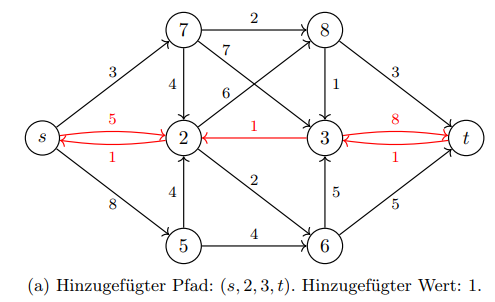
\includegraphics[width=8cm]{fordBsp1.png}}

\section{Baumoperationen}
    \subsection{BST}
        \subsubsection*{Löschen}
            \centerline{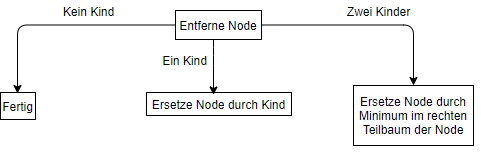
\includegraphics[width=10cm]{BSTDelete.png}}

    \subsection{RBT}
        \subsubsection*{Insert}
            \centerline{Wie im BST, neuen Knoten rot färben, danach FixUp:}
            \centerline{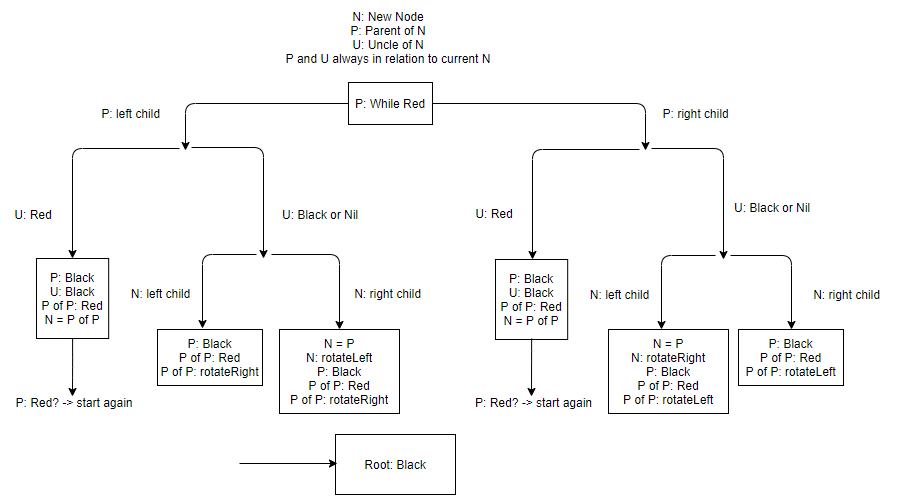
\includegraphics[width=15cm]{RBTInsert.png}}

    \subsection{AVL-Bäume}
        \subsubsection*{Einfügen/Löschen}
            \centerline{Einfügen und Löschen wie beim BST, danach jeweils Rebalancieren:}
            \centerline{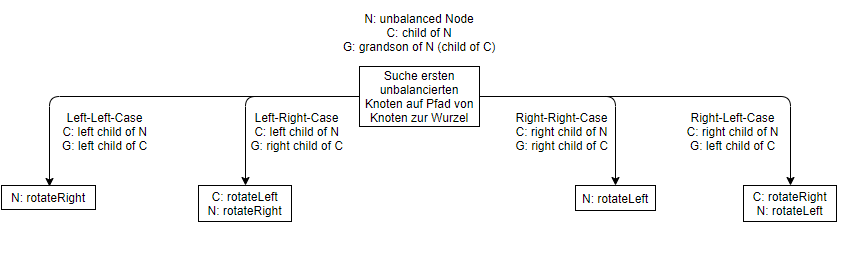
\includegraphics[width=15cm]{AVLRebalance.png}}
            Beachte beim Löschen: 
                \begin{itemize}
                    \item Wahl von C: größter Teilbaum von N (eindeutig, da N unbalanciert)
                    \item Wahl von G: größter Teilbaum von C (nicht eindeutig, Wahl Rechts-Rechts/Links-Links)
                    \item \textbf{Potenziell} müssen mehrere Knoten bearbeitet werden $\Rightarrow$ alle Knoten bis Wurzel prüfen
                \end{itemize}
\pagebreak
    \subsection{Splay-Bäume}
            \begin{itemize}
                \item Suchen: Spüle gesuchten Knoten an die Wurzel (alternativ zuletzt besuchten Knoten)
                \item Einfügen: Einfügen nach BST-Regeln und danach Hochspülen des Knotens
                \item Löschen:
                    \begin{itemize}
                        \item[1.] zu löschenden Knoten hochspülen
                        \item[2.] Knoten löschen
                        \item Falls nur ein Kind: Dieses Kind neue Wurzel und fertig
                        \item {\makebox[3cm][l]{Falls zwei Kinder:}}  Spüle größten Knoten im linken Teilbaum hoch
                        \item[] {\makebox[3cm][l]{}} Hänge danach beide Teilbäume an diesen Knoten
                    \end{itemize}
            \end{itemize}

        \subsubsection{Spülen}
            \centerline{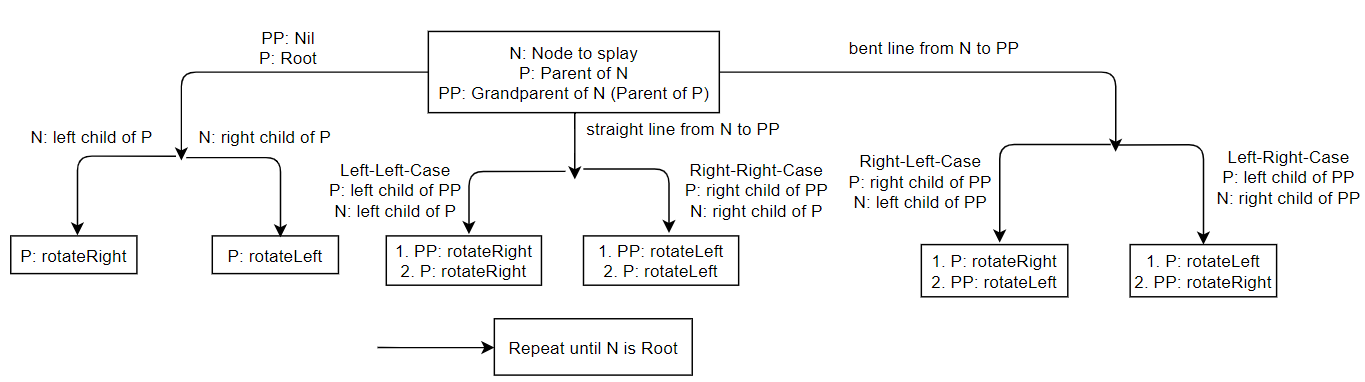
\includegraphics[width=15cm]{SplaySplay.png}}

    \subsection{Heaps}
        \subsubsection{Heap-Sort}
            \begin{enumerate}
                \item Array wird als Heap aufgefasst
                \item Heapeigenschaft wird wiederhergestellt (Heapify)
                \item Extrahieren der Wurzel (Maximum) und Ersetzen durch \string"letztes\string" Blatt
                \item Wieder Heapify um Wert an die richtige Stelle zu rücken
                \item Falls der Baum noch nicht leer ist, gehe zu Schritt 3
            \end{enumerate}

            \noindent
            Heapify: beginnend bei \texttt{ceil((H.length-1)/2) - 1} bis 0: vertausche nach unten, falls Parent kleiner als Child
            \centerline{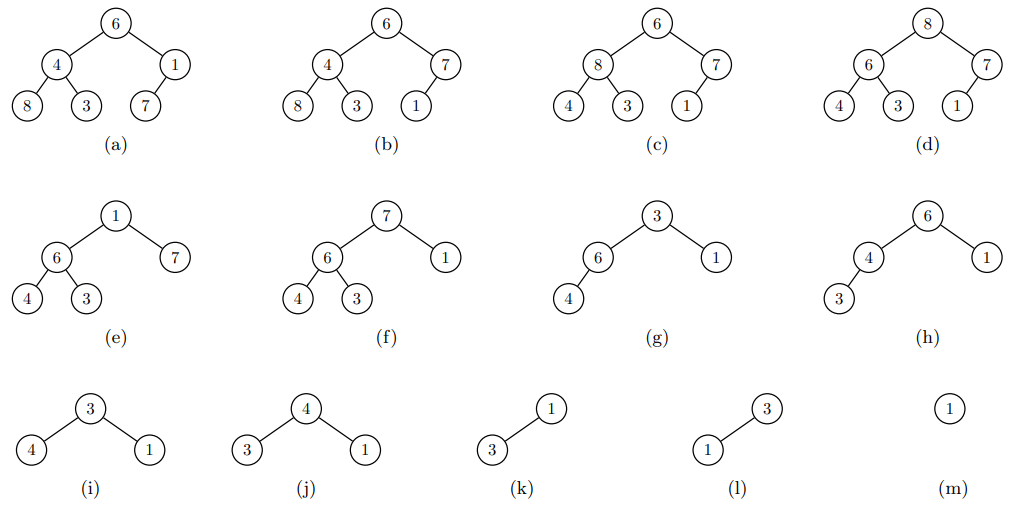
\includegraphics[width=15cm]{heapSortBsp.png}}

    \subsection{B-Bäume vom Grad \texttt{t}}
        \centerline{Knoten zwischen \texttt{[t-1, $\dots$,2t-1]} Werte (Wurzel: \texttt{[1, $\dots$,2t-1])}} 
        \subsubsection{Einfügen}
            \texttt{Split:}
                \begin{itemize}
                    \item Aufbrechen der vollen (\texttt{2t-1}) Node
                    \item Hinzufügen der mittleren Node zur Elternnode
                    \item Aus den anderen Nodes entstehen nun jeweils einzelne Kinder
                    \item Splitten an der Wurzel erzeugt neue Wurzel und erhöht Baumhöhe um 1
                \end{itemize}

            \centerline{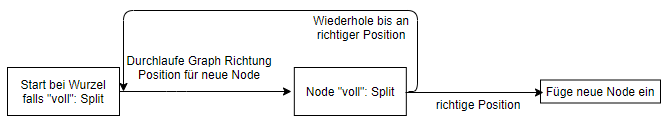
\includegraphics[width=15cm]{BInsert.png}}

        \subsubsection{Löschen}
            \begin{enumerate}
                \item Start bei Wurzel
                \item[] Wurzel: \texttt{1} Wert | Kinder der Wurzel: \texttt{t-1} Werte $\rightarrow$ Verschmelze Kinder und Wurzel
                \item Durchlaufe Graph von Node bis zum löschenden Knoten
                \item Überprüfe bei jeder Node:
                \item[]
                    \begin{minipage}{0.45\textwidth}
                        \textit{Verschmelzen} \\
                        Kind + Geschwister \texttt{t-1} Werte \\
                        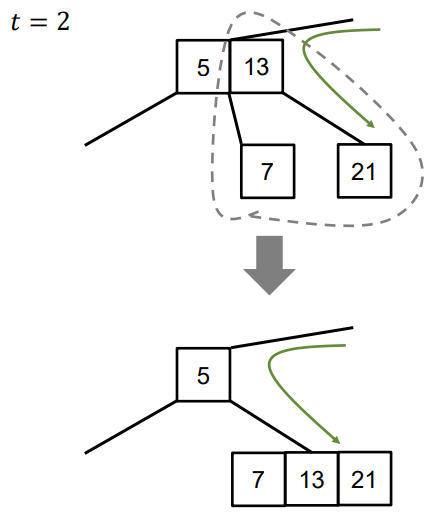
\includegraphics[width=4cm]{bbaumMelt.png}
                    \end{minipage} 
                    \begin{minipage}{0.45\textwidth}
                    \textit{Rotation} \\
                    Kind nur \texttt{t-1} Werte \\
                    Geschwister jedoch mehr als \texttt{t-1} Werte \\
                    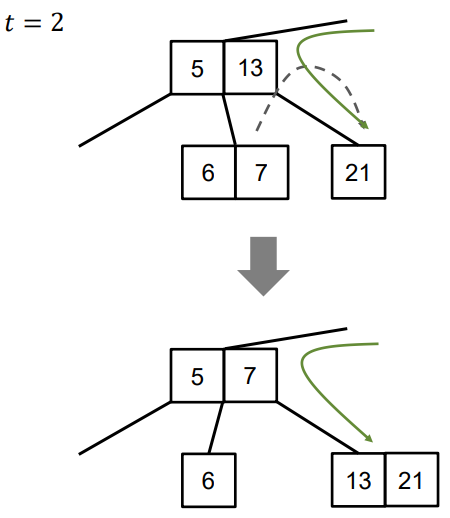
\includegraphics[width=4cm]{bbaumRot.png}
                    \end{minipage}
                \item Knoten gefunden:
                    \begin{itemize}
                        \item \textbf{Löschen im Blatt:} Einfach entfernen, fertig
                        \item \textbf{Löschen im inneren Knoten:}
                        \item[]
                            \begin{minipage}{0.4\textwidth}
                                \textit{Verschmelzen} \\
                                Beide Kinder \texttt{t-1} Werte \\
                                $\rightarrow$ Kindknoten verschmelzen \\
                                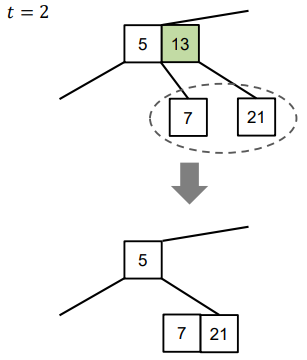
\includegraphics[width=4cm]{bbaumInnerMelt.png}
                            \end{minipage} 
                            \begin{minipage}{0.5\textwidth}
                            \textit{Verschieben} \\
                            Eines der Kinder mehr als \texttt{t-1} Werte \\
                            Größten Wert vom linken Kind nach oben kopieren oder \\
                            Kleinsten Wert vom rechten Kind nach oben kopieren\\
                            Potentiell rekursiv nach unten suchen \\
                            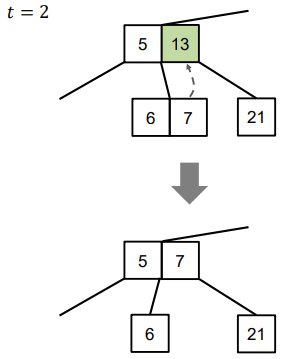
\includegraphics[width=4cm]{bbaumInnerRot.png}
                            \end{minipage}
                            \end{itemize}
            \end{enumerate}

\section{Randomized Data Structures}
    \subsection{Skip-Lists}
        \subsubsection{Einfügen}
            \begin{itemize}
                \item Suche richtige Position in unterster Liste
                \item Füge Wert ein
                \item Füge ihn auch in drüberliegende Skip-Lists ein, falls die zufällige Zahl $< p$ ist
            \end{itemize}
            \centerline{$p= \frac{1}{2}$, Zufallswerte: $0.33,0.82$ $\rightarrow$ 15 wird in eine höhere Skip-List eingefügt ($0.33 < \frac{1}{2}$, $0.82 > \frac{1}{2})$}
            \centerline{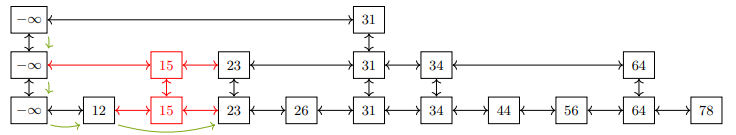
\includegraphics[width=15cm]{skipListsBsp.png}}

        \subsubsection{Löschen}
            \begin{itemize}
                \item Wert und alle Vorkommen in Expresslisten entfernen
            \end{itemize}

    \subsection{Hash-Tables}
        \begin{itemize}
            \item Abspeichern der Werte in einem Array anhand einer gewissen Hashfunktion
            \item Kollisionsauflösung z.B. mithilfe einer LinkedList
            \item Hashfunktion sollte gut verteilen und uniform sein
        \end{itemize}

    \subsection{Bloom-Filter}
        \begin{itemize}
            \item Speicherschonende Wörterbücher mit kleinem Fehler
            \item Erzeugen eines Bit-Arrays
            \item Bits werden anhand von verschiedenen Hash-Funktionen beim Einfügen neuer Werte auf 1 gesetzt
            \item Bei Überprüfung ob Wort im Filter: Überprüfen, ob alle Hashpositionen $= 1$ sind
        \end{itemize}

\section{Anwendungsbeispiele}
    \subsection{Sorting}

        \subsubsection{Insertion Sort}
        \centerline{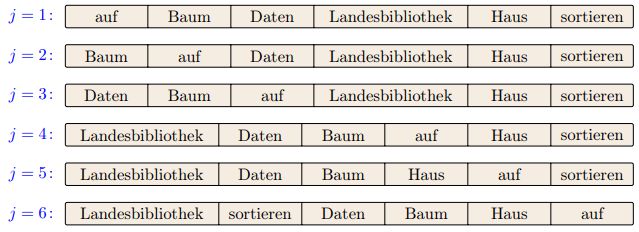
\includegraphics[width=12cm]{insertionSortBsp.png}}

        \subsubsection{Merge Sort}
        \centerline{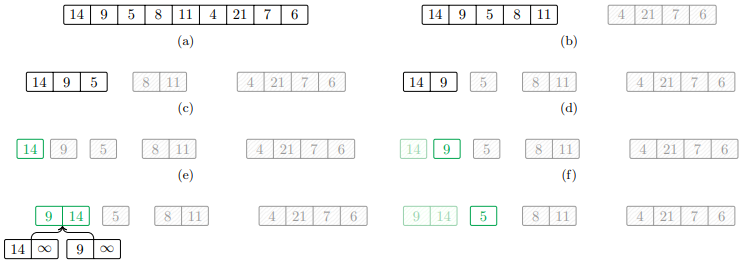
\includegraphics[width=12cm]{mergeSortBsp.png}}

        \subsubsection{Quick Sort}
        \centerline{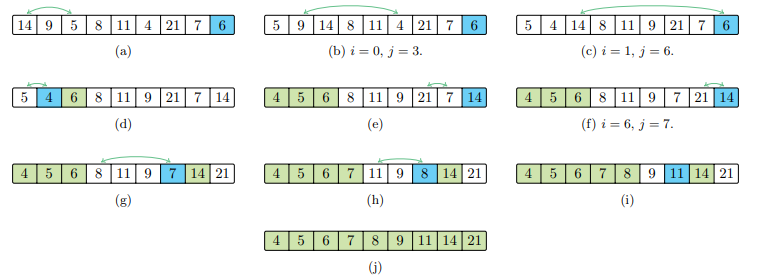
\includegraphics[width=12cm]{quickSortBsp.png}}

        \subsection{Basic Data Structures}

        \subsubsection{Stacks}
        \centerline{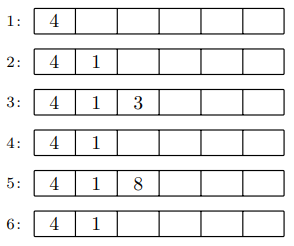
\includegraphics[width=5cm]{stackBsp.png}}

        \subsubsection{Queues}
        \centerline{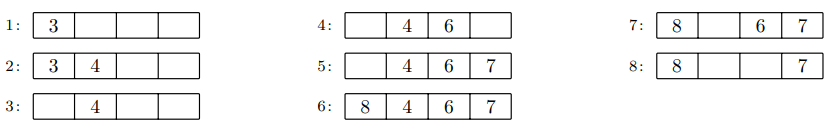
\includegraphics[width=12cm]{queueBsp.png}}

\pagebreak

\section{Pseudocode}
    \subsection{Sorting}
        \begin{ccode}[autogobble]{title=Insertion Sort(A)}  
            FOR j = 1 TO A.length - 1
            key = A[j]
            // Füge A[j] in die sortierte Sequenz A[0...j-1] ein
            i = j - 1
            WHILE i >= 0 and A[i] > key
                A[i + 1] = A[i]
                i = i - 1
            A[i + 1] = key
        \end{ccode}

        \begin{ccode}[autogobble]{title=BubbleSort(A)}  
            FOR i = 0 TO A.length - 2
                FOR j = A.length - 1 DOWNTO i + 1
                    IF A[j] < A[j-1]
                        SWAP(A[j], A[j-1])
            \end{ccode}
        
            \begin{ccode}[autogobble]{title=SelectionSort(A)}
            FOR i = 0 TO A.length - 2
                k = i 
                FOR j = i + 1 TO A.length - 1
                    IF A[j] < A[k]
                        k = j 
                SWAP(A[i], A[k])
            \end{ccode}
                
        \subsubsection{Quicksort}
            \begin{ccode}[autogobble,escapeinside=||]{title={QUICKSORT(A,p,r)}}
            IF p < r    // Überprüfung, ob Teilarray leer ist
                q = PARTITION(A,p,r)
                QUICKSORT(A,p,q-1)
                QUICKSORT(A,q+1,r)
            \end{ccode}
        
            \begin{ccode}[autogobble,escapeinside=||]{title={PARTITION(A,p,r)}}
            x = A[r]    // Wahl des Pivotelements
            i = p - 1   // Index i setzen
            FOR j = p TO r - 1 // Auffüllen des Teilarrays mit Elementen
                IF A[j] |$\leq$| x
                    i = i + 1
                    SWAP(A[i], A[j]) /
            SWAP(A[i+1], A[r]) // Tausch des Pivotelements
            RETURN i + 1 // Neuer Index des Pivotelements
            \end{ccode}

        \subsubsection{Merge Sort}
            \begin{ccode}[autogobble,escapeinside=||]{title={MergeSort(A, p, r)}}
            IF p < r
                q = |$\left \lfloor \texttt{(p+r)/2} \right \rfloor$| // Teilen in 2 Teilfolgen 
                MERGE-SORT(A,p,q) // Sortieren der beiden Teilfolgen
                MERGE-SORT(A,q+1,r)
                MERGE(A,p,q,r) // Vereinigung der beiden sortierten Teilfolgen
            \end{ccode}
        
            \begin{ccode}[autogobble,escapeinside=||]{title={MERGE(A,p,q,r)}}
            // Geteiltes Array an Stelle q
            |$n_1$| = q - p + 1
            |$n_2$| = r - q 
            Let L[0...|$n_1$|] and R[0...|$n_2$|] be new arrays 
            FOR i = 0 TO |$n_1$| - 1 // Auffüllen der neu erstellten Arrays
                L[i] = A[p + i]
            FOR j = 0 TO |$n_2$| - 1
                R[j] = A[q + j + 1]
            L[|$n_1$|] = |$\infty$| // Einfügen des Sentinel-Wertes
            R[|$n_2$|] = |$\infty$|
            i = 0
            j = 0
            FOR k = p TO r  // Eintragweiser Vergleich der Elemente          
                IF L[i] |$\leq$| R[j]
                    A[k] = L[i] // Sortiertes Zurückschreiben in Original-Array
                    i = i + 1
                ELSE 
                    A[k] = R[j]
                    j = j + 1
            \end{ccode}

    \subsection{Graphenalgorithmen}
        \subsubsection{Breadth-First Search}
            \begin{ccode}[autogobble, escapeinside=||]{title={BFS(G,s)}}
            FOREACH u in V-{s} DO
                u.color = WHITE;        // Weiß = noch nicht besucht
                u.dist = |$+\infty$|            // Setzen der Distanzen auf Unendlich
                u.pred = nil;           // Setzen der Vorgänger auf nil
            s.color = GRAY;             // Anfang bei Startnode
            s.dist = 0;
            s.pred = nil;
            newQueue(Q);
            enqueue(Q,s);
            WHILE !isEmpty(Q) DO
                u = dequeue(Q); 
                FOREACH v in adj(G,u) DO
                    IF v.color == WHITE THEN
                        v.color == GRAY;
                        v.dist = u.dist+1;
                        v.pred = u;
                        enqueue(Q,v);
                u.color = BLACK;            // Knoten abgearbeitet
            \end{ccode}

        \subsubsection{Depth-First Search}
            \begin{ccode}[autogobble, escapeinside=||]{title={DFS(G)}}
            FOREACH u in V DO
                u.color = WHITE;
                u.pred = nil;
            time = 0;               // time hier als globale Variable
            FOREACH u in v DO
                IF u.color == WHITE THEN
                    DFS-VISIT(G,u)  // Start eines rekursiven Aufrufs
            \end{ccode}

            \begin{ccode}[autogobble, escapeinside=||]{title={DFS-VISIT(G,u)}}
            time = time + 1;
            u.disc = time;          // discovery time
            u.color = GRAY;
            FOREACH v in adj(G,u) DO
                IF v.color == WHITE THEN
                    v.pred = u;
                    DFS-VISIT(G,v);
            u.color = BLACK;
            time = time + 1;
            u.finish = time;        // finish time
            \end{ccode}

    \subsection{Path-Finding Algorithmen}
        \subsubsection{Relax / initSSSP}
            \begin{ccode}[autogobble, escapeinside=||]{title={relax(G,u,v,w)}}
            IF v.dist > u.dist + w((u,v)) THEN
                v.dist = u.dist + w((u,v))
                v.pred = u
            \end{ccode}

            \begin{ccode}[autogobble, escapeinside=||]{title={initSSSP(G,s,w)}}
            FOREACH v in V DO
                v.dist = |$\infty$|
                v.pred = nil
            s.dist = 0
            \end{ccode}

        \subsubsection{Dijkstra}
            \begin{ccode}[autogobble, escapeinside=||]{title={Dijkstra-SSSP(G,s,w)}}
            initSSSP(G,s,w)
            Q = V
            WHILE !isEmpty(Q) DO
                u = EXTRACT-MIN(Q)
                FOREACH v in adj(u) DO
                    relax(G,u,v,w)
            \end{ccode}
        
        \subsubsection{Kürzester Pfad durch TopoSort bei DAG}
            \begin{ccode}[autogobble, escapeinside=||]{title={TopoSort-SSSP(G,s,w)}}
            initSSSP(G,s,w)
            execute topological sorting
            FOREACH u in V in topological order DO
                FOREACH v in adj(u) DO
                    relax(G,u,v,w)
            \end{ccode}

        \subsubsection{Bellmann-Ford-Algorithmus}
            \begin{ccode}[autogobble, escapeinside=||]{title={Bellmann-Ford-SSSP(G,s,w)}}
            initSSSP(G,s,w)

            FOR i = 1 TO V - 1 DO
                FOREACH (u,v) in E DO
                    relax(G,u,v,w)
            FOREACH (u,v) in E DO   // checks if negative cycle exists
                IF v.dist > u.dist + w((u,v)) THEN
                    RETURN FALSE
            RETURN TRUE
            \end{ccode}
            
    \subsection{Minimale Spannbäume}
            
        \subsubsection{Kruskal}
            \begin{ccode}[autogobble, escapeinside=||]{title={MST-Kruskal(G,w)}}
            A = |$\emptyset$|
            FOREACH v in V DO
                set(v) = {v};       // Menge mit sich selbst
            Sort edges according to weight in increasing order
            FOREACH {u,v} in E according to order DO
                IF set(u) |$\neq$| set(v) THEN     // Mengen noch nicht verbunden
                    A = A |$\cup$| {{u,v}}
                    UNION(G,u,v)   // Zusammenführen der Mengen aller Knoten aus Sets
            RETURN A
            \end{ccode}

        \subsubsection{Prim}
            \begin{ccode}[autogobble, escapeinside=||]{title={MST-Prim(G,w,r)}}
            // r is given root
            FOREACH v in V DO
                v.key = |$+\infty$|
                v.pred = nil
            r.key = |$-\infty$|
            Q = V
            WHILE !isEmpty(Q) DO
                u = EXTRACT-MIN(Q)
                FOREACH v in adj(u) DO
                    IF v |$\in$| Q and w({u,v}) THEN
                        v.key = w({u,v})
                        v.pred = u
            \end{ccode}
        
    \subsection{Netzwerkflüsse - Ford-Fulkerson}
            \begin{ccode}[autogobble, escapeinside=||]{title={Ford-Fulkerson(G,s,t,c)}}
            FOREACH e in E do e.flow = 0;
            WHILE there is path p from s to t in |$G_{flow}$| DO
                |$c_{flow}(p)$| = min {|$c_{flow}(u,v)$| : (u,v) in p}
                FOREACH e in p DO
                    IF e in E THEN
                        e.flow = e.flow + |$c_{flow}(p)$|;
                    ELSE
                        e.flow = e.flow - |$c_{flow}(p)$|;
            \end{ccode}

\section{Laufzeitentabelle}

\begin{table}[h]
\scriptsize
\begin{tabularx}{\textwidth}{l | X X X X | X X X X | l}
    \toprule

    \textbf{Data Str.} & \multicolumn{8}{c|}{\textbf{Time Complexity}} & \textbf{Space Complexity} \\
    \midrule
    & \multicolumn{4}{l|}{\textbf{Average Case}} & \multicolumn{4}{l|}{\textbf{Worst Case}} & \textbf{Worst Case} \\ 
    \midrule
    & \textit{Access} & \textit{Search} & \textit{Insert} & \textit{Delete} & \textit{Access} & \textit{Search} & \textit{Insert} & \textit{Delete} & \\
    \midrule
    Array & $\Theta(1)$ & $\Theta(n)$ & $\Theta(n)$ & $\Theta(n)$ & $O(1)$ & $O(n)$ & $O(n)$ & $O(n)$ & $O(n)$ \\
    \midrule
    Stack & $\Theta(n)$ & $\Theta(n)$ & $\Theta(1)$ & $\Theta(1)$ & $O(n)$ & $O(n)$ & $O(1)$ & $O(1)$ & $O(n)$ \\
    \midrule
    Queue & $\Theta(n)$ & $\Theta(n)$ & $\Theta(1)$ & $\Theta(1)$ & $O(n)$ & $O(n)$ & $O(1)$ & $O(1)$ & $O(n)$ \\
    \midrule
    LinkedList & $\Theta(n)$ & $\Theta(n)$ & $\Theta(1)$ & $\Theta(1)$ & $O(n)$ & $O(n)$ & $O(1)$ & $O(1)$ & $O(n)$ \\
    \midrule
    BST & $\Theta(\log n)$ & $\Theta(\log n)$ & $\Theta(\log n)$ & $\Theta(\log n)$ & $O(n)$ & $O(n)$ & $O(n)$ & $O(n)$ & $O(n)$ \\
    \midrule
    RBT & $\Theta(\log n)$ & $\Theta(\log n)$ & $\Theta(\log n)$ & $\Theta(\log n)$ & $O(\log n)$ & $O(\log n)$ & $O(\log n)$ & $O(\log n)$  & $O(n)$ \\
    \midrule
    Splay & / & $\Theta(\log n)$ & $\Theta(\log n)$ & $\Theta(\log n)$ & / & $O(\log n)$ & $O(\log n)$ & $O(\log n)$  & $O(n)$ \\
    \midrule
    AVL & $\Theta(\log n)$ & $\Theta(\log n)$ & $\Theta(\log n)$ & $\Theta(\log n)$ & $O(\log n)$ & $O(\log n)$ & $O(\log n)$ & $O(\log n)$  & $O(n)$ \\
    \midrule
    B-Tree & $\Theta(\log n)$ & $\Theta(\log n)$ & $\Theta(\log n)$ & $\Theta(\log n)$ & $O(\log n)$ & $O(\log n)$ & $O(\log n)$ & $O(\log n)$  & $O(n)$ \\
    \midrule
    Skip-List & $\Theta(\log n)$ & $\Theta(\log n)$ & $\Theta(\log n)$ & $\Theta(\log n)$ & $O(n)$ & $O(n)$ & $O(n)$ & $O(n)$ & $O(n \log n)$ \\
    \midrule
    Hash-Table & / & $\Theta(1)$ & $\Theta(1)$ & $\Theta(1)$ & / & $O(n)$ & $O(n)$ & $O(n)$ & $O(n)$ \\
    \bottomrule
\end{tabularx}
\end{table}

\begin{table}[h]
    \scriptsize
    \begin{tabularx}{\textwidth}{l | X X X X | l}
        \toprule
    
        \textbf{Algorithm} & \multicolumn{3}{c|}{\textbf{Time Complexity}} & \textbf{Space Complexity} \\
        \midrule
        & \textbf{Best Case} &\textbf{Average Case} & \textbf{Worst Case} & \textbf{Worst Case} \\ 
        \midrule
        Insertion Sort & $\Omega(n)$ & $\Theta(n^2)$ & $O(n^2)$ & $O(1)$ \\
        \midrule
        Bubble Sort & $\Omega(n)$ & $\Theta(n^2)$ & $O(n^2)$ & $O(1)$ \\
        \midrule
        Selection Sort & $\Omega(n^2)$ & $\Theta(n^2)$ & $O(n^2)$ & $O(1)$ \\
        \midrule
        Merge Sort & $\Omega(n \log n)$ & $\Theta(n \log n)$ & $O(n \log n)$ & $O(n)$ \\
        \midrule
        Quick Sort & $\Omega(n \log n)$ & $\Theta(n \log n)$ & $O(n^2)$ & $O(\log n)$ \\
        \midrule
        Heap Sort & $\Omega(n \log n)$ & $\Theta(n \log n)$ & $O(n \log n)$ & $O(1)$ \\
        \midrule

    \end{tabularx}
    \end{table}

\pagebreak

\section{MasterTheorem - Beispiele}
    \centerline{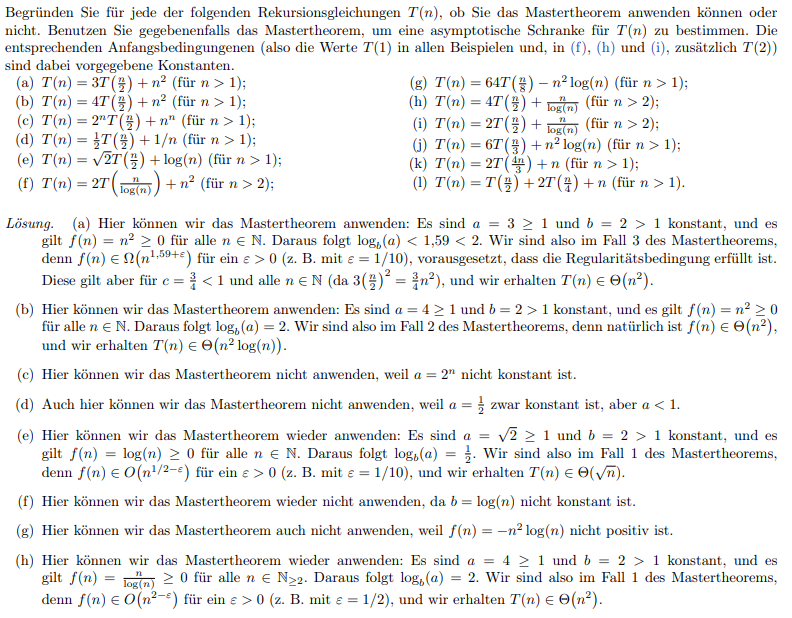
\includegraphics[width=15cm]{masterTheoremBsp1.png}}
    \centerline{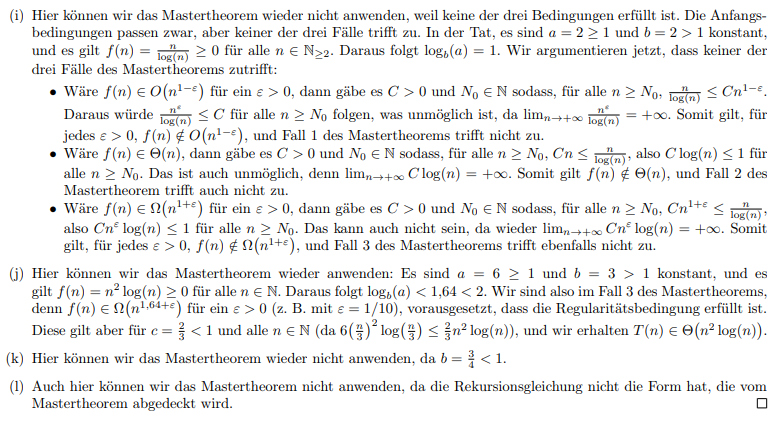
\includegraphics[width=15cm]{masterTheoremBsp2.png}}
    
\end{document}